%!TEX root = ../main.tex
I dette afsnit ses de forskellige Use cases. På figur~\ref{fig:fullydressedusecases} vises et use-case diagram over de fully-dressed use-cases, som viser de use-cases, som er i fokus. På figur~\ref{fig:ikkefullydressedusecases} vises et use-case diagram over de ikke fully-dressed use-cases, som ønskes implementeret på et senere tidspunkt. 
\begin{figure}[ht]
	\centering
	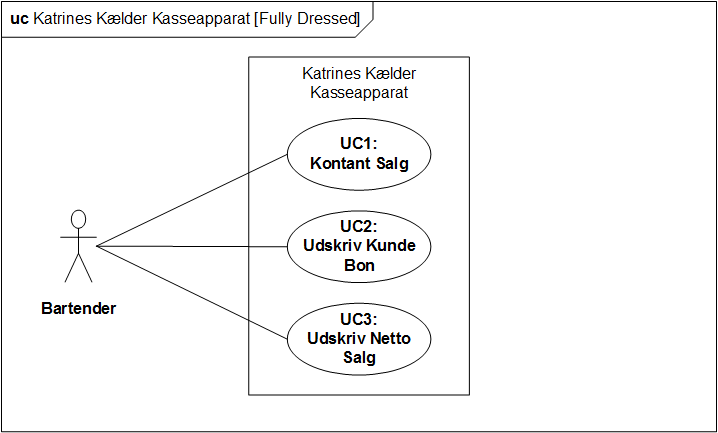
\includegraphics[width=0.8\textwidth]{Kravspecifikation/UseCases/UseCases_fully_dressed.png}
	\caption{Use-case diagram for de fully dressed use-cases.}
	\label{fig:fullydressedusecases}
\end{figure}

\begin{figure}[ht]
	\centering
	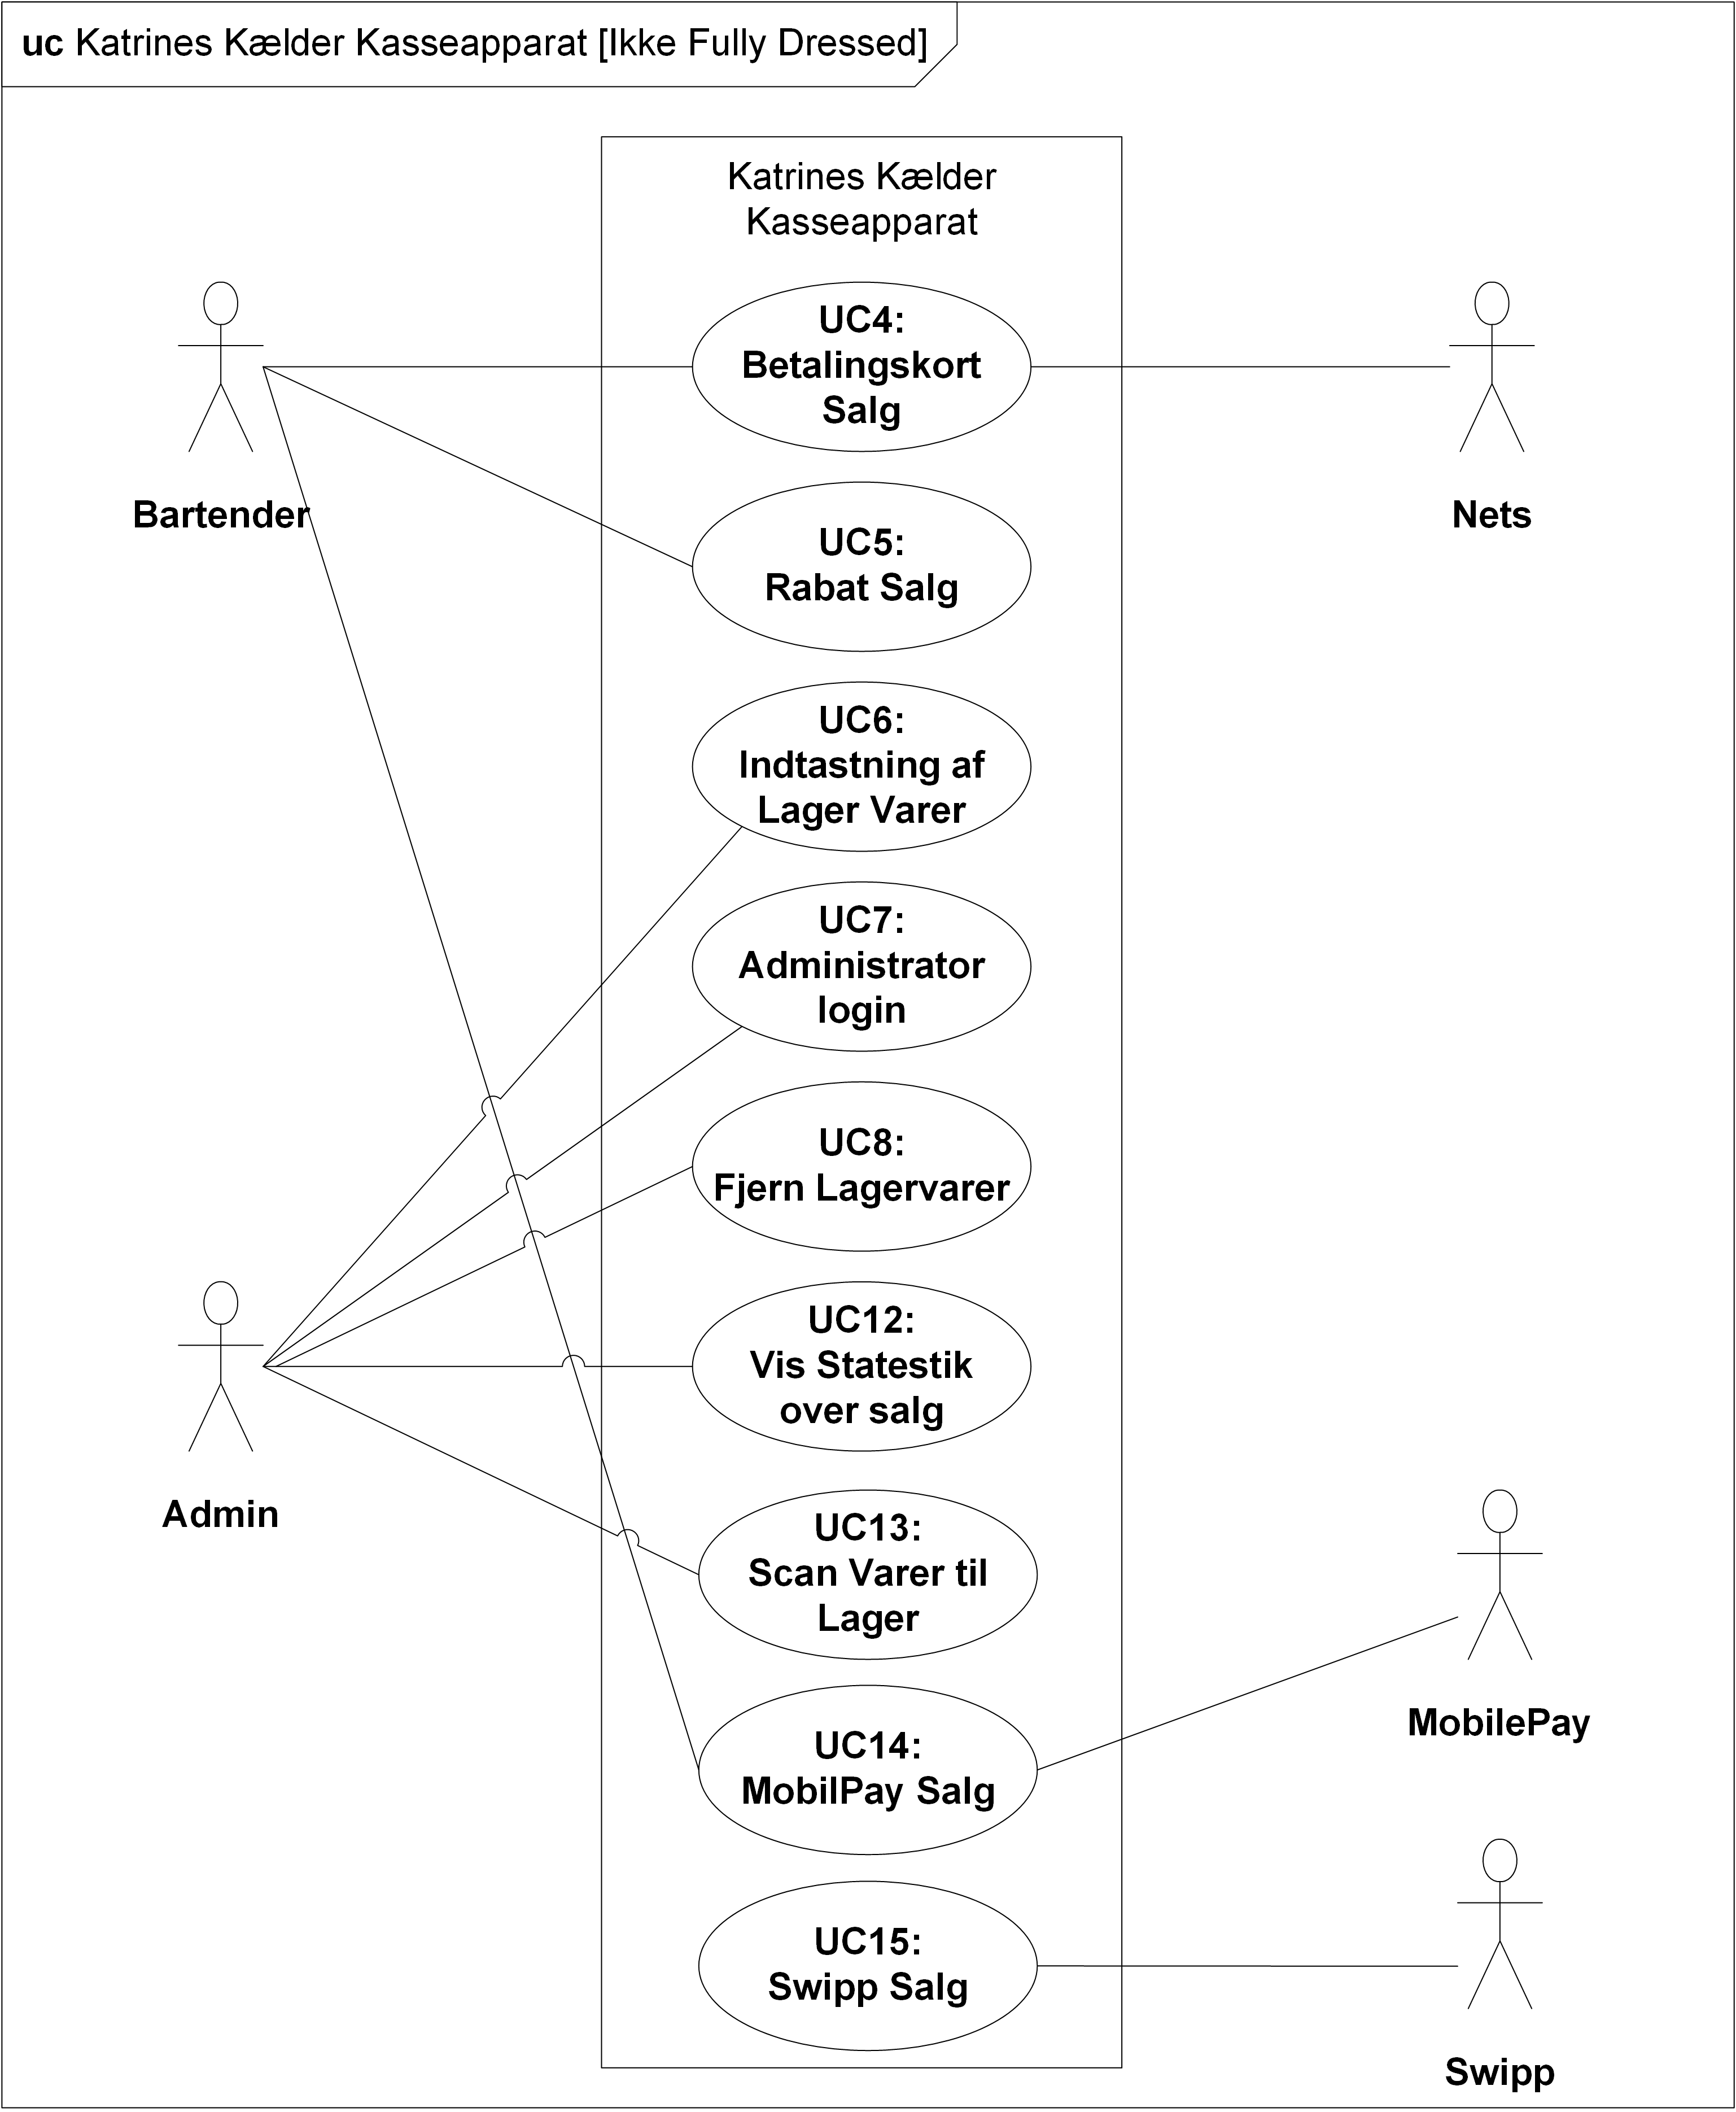
\includegraphics[width=0.8\textwidth]{Kravspecifikation/UseCases/UseCases_not_fully_dressed.png}
	\caption{Use-case diagram for de ikke fully dressed use-cases.}
	\label{fig:ikkefullydressedusecases}
\end{figure}
\newpage

%!TEX root = ../../main.tex

\subsection*{Use case 1}
I denne use case ser vi hvor et kontant salg bliver foretaget
\begin{usecase}{1}

\title{ Kontant Salg } 

\field{Mål:}{ At sælge drikkevarer mod kontant betaling }

\field{Initieret af:}{ Bartender }

\field{Aktører:}{ Bartender }

\field{Samtidige forekomster:}{1}

%Preconditions: What must be true on start and worth telling the reader?
\field{Prækondition:}{System skal være tændt og klar}

%Postconditions: What must be true on successful completion and worth telling the reader
\field{Postkondition:}{ Et kontant salg er foretaget }

%Main Success Scenario: A typical, unconditional happy path scenario of success.
\scenario{Hovedscenarie:}{
	\item Bartender vælger drink(s)/pris(er) på systemets touchskærm
	\item Bartender trykker "Total"	
	\item Den samlede pris udregnes
	\item Bartender trykker "Kontant" og skuffen åbnes
	\item Bartender modtager betaling fra kunden
	[Extension 1.1: Kontanter ikke modtaget]
	\item Købet er afsluttet
}


%Extensions: Alternate scenarios of success or failure.
\scenario{Extension 1.1: Kontanter ikke modtaget:}{
		\item Bartender trykker annuller køb
		\item Bartender lukker skuffen
		\item Systemet er klar til næste kunde
}


\end{usecase}



%!TEX root = ../../main.tex

\subsection*{Use case 1}
I denne use case -----
\begin{usecase}

\addtitle{Use Case 2}{ Udskriv Kundebon } 

\addfield{Mål:}{ Systemet får udskrevet en bon med kundens køb på }

\addfield{Initieret af:}{ Bartender }

\addfield{Aktører:}{ Bartender (Primær) }

\addfield{Samtidige forekomster:}{1}

%Preconditions: What must be true on start and worth telling the reader?
\addfield{Prækondition:}{Use Case 1 er gennemført}

%Postconditions: What must be true on successful completion and worth telling the reader
\addfield{Postkondition:}{Kunden (baretender?) modtager bon med køb på }

%Main Success Scenario: A typical, unconditional happy path scenario of success.
\addscenario{Hovedscenarie:}{
	\item Bartender har valgt at der skal udskrives bon (på GUI?)
	\item En dialogbox popper op og bartender bekræfter ønske af bon	
	\item printer udskriver bon  [Ext 1: Der er ikke mere papir]
	\item Bartender udleverer bon til kunde [Ext 2: Kunde er gået]	
}

%Extensions: Alternate scenarios of success or failure.
\addscenario{Udvidelser:}{
	\item[Ex.1] Der er ikke mere papir
		\begin{enumerate}
		\item[1.] Printer stopper. Dialogbox popper op med besked "Fyld papir på printer"
		\item[2.] Bartender fylder papir på printer.
		\item[3.] Der trykkes på 'OK' og fortsættes fra punkt 3
		\end{enumerate}
	\item[Ex.2] Kunde er gået
		\begin{enumerate}
			\item[1.] Bartender smider bon ud
		\end{enumerate}
}


\end{usecase}


\section{Ikke fully dressed use cases}

\subsubsection*{Use Case 4 - Dankort Salg}
skal beskrive forløbet for et salg når kasseapparatet interagerer med dankort automaten.

\subsubsection*{Use Case 5 - Medarbejder Salg}
Heri beskrives forløbet for salg til en medarbejder der opnår rabat.

\subsubsection*{Use Case 6 - Indtastning af lager varer}
Til lagerstyrings delen af produktet skal der være mulighed for at indtaste vare i systemet når de ankommer/bestilles.

\subsubsection*{Use Case 7 - Admin login}
For at kunne ændre priser, indsætte nye varer osv. skal der kunne logges ind på en administrationsdel af systemet således at ikke alle og enhver kan gøre dette.

\subsubsection*{Use Case 8 - Fjern lagervarer}
Når der hentes varer på lageret skal disse kunne tjekkes ud af systemet.

\subsubsection*{Use Case 9 - Tilføj varer til kasseapparat}
Det skal være muligt at tilføje en varer til kasseapparatet denne use case kræver at admin login use casen er udført.

\subsubsection*{Use Case 10 - Rediger varer i kasseapparat}
Det skal være muligt at ændre en varers pris og navn osv. denne use case kræver admin login use casen er udført.

\subsubsection*{Use Case 11 - Fjern varer fra kasseapparat}
Det skal være muligt at fjerne drinks fra systemet hvis de f.eks. ikke længere bliver serveret. denne use case kræver admin login use casen er udført.

\subsubsection*{Use Case 12 - Vis Statistik over salg}
Der skal kunne generes en statistik over de varer der er blevet solgt gerne i detaljer der specifikt beskriver hvilke drinks der er solgt.

\subsubsection*{Use Case 13 - Scan varer til lager}
Der skal kunne bruges et apparat der kan scanne varer ind i lager systemet. 